\section{Beam Elements}
\label{sec:beams}

From the mechanics of materials beam theory, the shear stress $V$ in a beam is related to the vertical distributed load $f_y(x)$ as shown by Equation~\ref{eq:shear_vertical_load}:

\begin{equation}
  \label{eq:shear_vertical_load}
  \frac{dV}{dx} = f_y(x)
\end{equation}

Let $v(x)$ be the vertical displacement of the beam's centroidal axis.
Then, the bending moment $M(x)$ can be expressed in terms of this displacement (Equation~\ref{eq:beam_bending_moment}):

\begin{equation}
  \label{eq:beam_bending_moment}
  M(x) = E I \frac{d^2v(x)}{dx^2}
\end{equation}

The relationship between the shear stress $V(x)$ and the bending moment $M(x)$ is given by Equation~\ref{eq:shear_bending_relation}:

\begin{equation}
  \label{eq:shear_bending_relation}
  V(x) = \frac{dM(x)}{dx} = \frac{d}{dx} \left( E I \frac{d^2v(x)}{dx^2} \right)
\end{equation}

And hence, the beam's governing differential equation, provided $EI$ is constant, is given by Equation~\ref{eq:beam_governing_eq}:

\begin{equation}
  \label{eq:beam_governing_eq}
  E I \frac{d^4v(x)}{dx^4} = f_y(x)
\end{equation}


\subsection{Energy Formulation}

Energy...


\subsection{Displacement Field And Interpolation Functions}

The vector $\left\{ q^e \right\}$ contains the beam finite element start and end nodes vertical displacements and rotations:

\[
  \left\{ q^e \right\} =
  \begin{Bmatrix}
    v_1 \\
    \theta_1 \\
    v_2 \\
    \theta_2 \\
  \end{Bmatrix} =
  \begin{Bmatrix}
    v_1 \\
    \left( \frac{dv}{dx} \right)_1 \\
    v_2 \\
    \left( \frac{dv}{dx} \right)_2 \\
  \end{Bmatrix}
\]

Let $v(x)$ be the vertical displacements field in the beam finite element of length $L$.
We can assume a cubic displacement field inside the element, as described by Equation~\ref{eq:beam_disp_field}:

\begin{equation}
  \label{eq:beam_disp_field}
  v(x) = N_1 v_1 + N_2 \theta_1 + N_3 v_2 + N_4 \theta_2
\end{equation}

where:

\begin{equation}
  \begin{split}
    N_1(x) & = \frac{1}{L^3} \left( 2x^3 -3x^2L + L^3 \right) \\
    N_2(x) & = \frac{1}{L^2} \left( x^3 - 2x^2L + xL^2 \right) \\
    N_3(x) & = \frac{1}{L^3} \left( -2x^3 - 3x^2L \right) \\
    N_4(x) & = \frac{1}{L^2} \left( x^3 - x^2L \right) \\
  \end{split}
\end{equation}

These N interpolation functions fulfill the following conditions:

\[
  \begin{aligned}
    N_1(0) & = 1    &    N_1'(0) & = 0    &    N_1(L) & = 0    &    N_1'(L) & = 0 \\
    N_2(0) & = 0    &    N_2'(0) & = 1    &    N_2(L) & = 0    &    N_2'(L) & = 0 \\
    N_3(0) & = 0    &    N_3'(0) & = 0    &    N_3(L) & = 1    &    N_3'(L) & = 0 \\
    N_4(0) & = 0    &    N_4'(0) & = 0    &    N_4(L) & = 0    &    N_4'(L) & = 1 \\
  \end{aligned}
\]

The displacement field can be rewritten as:

\[
  v(x) = \left[ N \right] \left\{ q^e \right\} =
  \begin{bmatrix}
    N_1 & N_2 & N_3 & N_4 \\
  \end{bmatrix}
  \begin{Bmatrix}
    v_1 \\
    \theta_1 \\
    v_2 \\
    \theta_2 \\
  \end{Bmatrix}
\]


\subsection{Distributed Loads}

Considering the distributed load formulation as in Equation~\ref{eq:distributed_linear_load}, but in the y direction $q_y(x)$, the work done by the load is:

\[
  W_{q_y} = \int_0^L q_y(x) \vec{v}(x) dx
\]
which yields a result of:

\[
  W_{q_y} = 
  \begin{bmatrix}    
    \frac{aL}{2} + \frac{3 L^2 b}{20} & \frac{aL^2}{12} + \frac{bL^3}{30} & \frac{aL}{2} + \frac{7bL^2}{20} & -\frac{aL^2}{12} - \frac{bL^3}{20} \\
  \end{bmatrix}
  \begin{Bmatrix}
    v_1 \\
    \theta_1 \\
    v_2 \\
    \theta_2 \\
  \end{Bmatrix}
\]

Therefore, a linear load $q_y(x)$ can be distributed over the two nodes in the finite element adding the forces and moments:

\begin{equation}
  \begin{split}
    F_y^1 = & \frac{aL}{2} + \frac{3 L^2 b}{20} \\
    M_z^1 = & \frac{aL^2}{12} + \frac{bL^3}{30} \\
    F_y^2 = & \frac{aL}{2} + \frac{7bL^2}{20} \\
    M_z^2 = & -\frac{aL^2}{12} - \frac{bL^3}{20} \\
  \end{split}
\end{equation}

Figure~\ref{fig:beam_finite_element_load_distribution} depicts this distibution of a linear shear load inside a finite element of length L.

\begin{figure}[h]
  \label{fig:beam_finite_element_load_distribution}
  \centering
  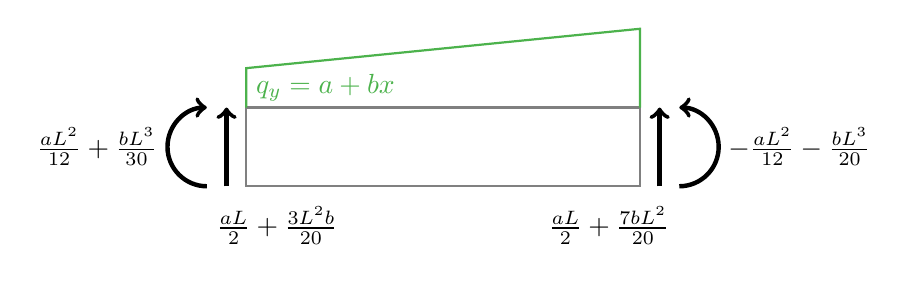
\begin{tikzpicture}
    \draw[gray, thick] (1,0) rectangle (6,1);
    \draw[green!40!gray, thick] (1,1) -- (1,1.5) -- (6,2) -- (6,1);
    \filldraw[green!40!gray] (1,1.25) node[anchor=west] {$q_y = a + bx$};
   
    \draw[ultra thick, ->] (0.75,0) -- (0.75, 1);
    \filldraw[black] (0.5, -0.5) node[anchor=west] {$\frac{aL}{2} + \frac{3 L^2 b}{20}$};  
    
    \draw[ultra thick, ->] (0.5,0) arc (-90:-270:0.5);
    \filldraw[black] (0, 0.5) node[anchor=east] {$\frac{aL^2}{12} + \frac{bL^3}{30}$};  
    
    \draw[ultra thick, ->] (6.25,0) -- (6.25, 1);
    \filldraw[black] (6.5,-0.5) node[anchor=east] {$\frac{aL}{2} + \frac{7bL^2}{20}$};  
    
    \draw[ultra thick, ->] (6.5,0) arc (-90:90:0.5);
    \filldraw[black] (7,0.5) node[anchor=west] {$-\frac{aL^2}{12} - \frac{bL^3}{20}$};  
  \end{tikzpicture}
  \caption{Distribution of a distributed shear load}
\end{figure}


\subsection{Shear Force}

Given the expression for the shear force $V(x)$ function of the displacement field $v(x)$:

\begin{equation}
  V(x) = \frac{d}{dx} \left( EI \frac{d^2v}{dx^2} \right)
\end{equation}
and knowing that $v(x)$ is:

\begin{equation}
  \label{eq:vertical_disp_field}
  v(x) = 
  \left[ \frac{2}{L^3} \left( v_1 - v_2 \right) + \frac{1}{L^2} \left( \theta_1 + \theta_2 \right) \right] x^3
  + \left[ \frac{-3}{L^2} \left( v_1 - v_2 \right) - \frac{1}{L} \left( 2 \theta_1 + \theta_2 \right) \right] x^2
  + \theta_1 x + v_2
\end{equation}
The shear force inside the element $V_e$ is then:

\[
  V_e = \frac{12EI}{L^3} \left( v_1 - v_2 \right) + \frac{6EI}{L^2} \left( \theta_1 + \theta_2 \right)
\]

Given the shear force inside the element, $V_e$, we can compute the values for the shear force in the element nodes:

\[
  \begin{split}
    V_e^1 = V_e - F_y^1 \\
    V_e^2 = V_e + F_y^2 \\
  \end{split}  
\]


\subsection{Bending Moment}

Given the expression for the bending moment $M(x)$ function of the displacement field $v(x)$:

\begin{equation}
  M(x) = EI \frac{d^2v}{dx^2}
\end{equation}
and the vertical displacement field expression in Formula~\ref{eq:vertical_disp_field}, the bending moment can be computed as follows:

\[
  M(x)  = EI \left( \frac{12x - 6L}{L^3} v_1 + \frac{6x - 4L}{L^2} \theta_1 + \frac{-12x + 6L}{L^3} v_2 + \frac{6x - 2L}{L^2} \theta_2 \right)
\]
Evaluating this equation for $x = 0$ and $x = L$, we obtain:

\[
  \begin{split}
    M(0) = \frac{6EI}{L^2} (v_2 - v_1) - \frac{2EI}{L} (\theta_2 + 2 \theta_1) \\
    M(L) = \frac{6EI}{L^2} (v_1 - v_2) + \frac{2EI}{L} (\theta_1 + 2 \theta_2) \\
  \end{split}  
\]

And finally, accounting for the external bending moments in the nodes, we can compute the bending moment values for the nodes of the finete element as follows:

\[
  \begin{split}
    M_e^1 = M(0) + M_z^0 \\
    M_e^2 = M(L) - M_z^1 \\
  \end{split}  
\]
